\documentclass[t]{beamer}

% Load general definitions
% Preamble file - general definitions, package loading, etc.

%=================================
% Load packages
\usepackage{amssymb,amsmath}
\usepackage{graphicx}
\usepackage{url}
\usepackage{tikz}
\usetikzlibrary{mindmap,trees,arrows}
\usepackage{fancyvrb}
\usepackage[portuguese]{babel} 
\usepackage[utf8]{inputenc}
\usepackage{subfigure}
\usepackage{times}
\usepackage[T1]{fontenc}
\usepackage{cancel}
\usepackage{color}
\usepackage{listings}
\usepackage[document]{ragged2e}
\usepackage{hyperref}
\usepackage{listings}


%=================================
% Set mode
\mode<presentation>
{
	\usetheme{Madrid}
	\usecolortheme{structure}
	\useoutertheme{infolines}
	\setbeamercovered{invisible}
}

% Get rid of nav bar
\beamertemplatenavigationsymbolsempty

% Insert frame number at bottom of the page.
\usefoottemplate{\hfil\tiny{\color{black!90}\insertframenumber}} 

%=================================
% Define new commands

\newcommand\Real{{\mathbb{R}}}
%\newcommand{\vi}{\vspace{0.6\baselineskip}}
%\newcommand{\goodgap}{\hspace{\subfigtopskip}\hspace{\subfigbottomskip}}


% Equation environments
\newcommand{\beq}{\begin{equation}}
\newcommand{\eq}{\end{equation}}
\newcommand{\beqs}{\begin{equation*}}
\newcommand{\eqs}{\end{equation*}}
\newcommand{\beqn}{\begin{eqnarray}}
\newcommand{\eqn}{\end{eqnarray}}
% Bold variables
\newcommand{\mbf}[1]{\ensuremath{\mathbf{#1}}}
% Itemization
\newcommand{\bitem}{\begin{itemize}}
\newcommand{\eitem}{\end{itemize}}
\newcommand{\spitem}{\vskip 1em\item}
\newcommand{\bitems}{\begin{itemize}\item}
\newcommand{\benums}{\begin{enumerate}\item}
\newcommand{\eenum}{\end{enumerate}}
% color blocks
\newenvironment{colorblock}[2]{%
\setbeamercolor{block title}{#2}
\begin{block}{#1}}{\end{block}}
% Vertical spacing
\newcommand{\vone}{\vskip 1em}
\newcommand{\vhalf}{\vskip .5em}
% Frame environments
\newenvironment{ftst}[3][t]{%
\begin{frame}{environment=ftst,#1}
\frametitle{#2}
\framesubtitle{#3}}{\end{frame}}
\newenvironment{ftstf}[2]{
\begin{frame}[fragile,environment=ftstf]
\frametitle{#1}
\framesubtitle{#2}}{\end{frame}}
% colors
\definecolor{MyGray}{rgb}{0.5,0.5,0.5}
\definecolor{MyDBGray}{rgb}{0.1,0.1,0.4}
\definecolor{darkgreen}{rgb}{0,0.4,0}
\definecolor{black}{rgb}{0,0,0}
\def\defn#1{{\color{red} #1}}
% Footnote
\renewcommand{\thefootnote}{\alph{footnote}}
% Relaxed footnotes
\newcommand{\lfr}[1]{\let\thefootnote\relax\footnote{\tiny #1}}
% Verbatim environment - using FANCYVRB package
\DefineVerbatimEnvironment%
{rcode}{Verbatim}
{fontsize=\scriptsize}

% Verbatim environment - using LISTINGS package
%\lstnewenvironment{rcode} {\lstset{	language = R,
%									basicstyle = \scriptsize\ttfamily,
%									showspaces = false,
%									showstringspaces = false,
%									showtabs = false,
%									keywordstyle = \color{black}\bfseries,
%									commentstyle = \color{darkgreen},
%									numbers = none,
%									otherkeywords={	<-,
%													ggplot,
%													geom_boxplot,
%													facet_grid,
%													shapiro.test,
%													fligner.test,
%													glht,
%													with},
%									deletekeywords={data,
%													model,
%													residuals,
%													c,
%													axis,
%													default,
%													labels,
%													qq.text}}}%
%{}

% Specific definitions
\title[]{Tópicos Especiais em Computação I}
\subtitle[]{Aprendizado Estatístico}
\author[]{Patrícia Lucas\\{\footnotesize }}
\institute{Bacharelado em Sistemas de Informação \\ IFNMG  - Campus Salinas}
\date{\scriptsize Salinas\\Março 2021}

\begin{document}

\setbeamertemplate{caption}{\raggedright\insertcaption\par}
% cover page
\setbeamertemplate{footline}{}
\begin{frame}

\begin{center}
\includegraphics[width=.15\textwidth]{}
\end{center}
  \titlepage
  \begin{tikzpicture}[remember picture,overlay]
  \node[anchor=south east,xshift=-5pt,yshift=5pt] at (current page.south east) {\tiny Versão 1.2021};
  \node[anchor=south west,yshift=0pt] at (current page.south west) {
\includegraphics[width=.25\textwidth]{Logos/salinas_horizontal_jpg.jpg}};
  \end{tikzpicture}  
\end{frame}

% Main slides

\begin{ftst}{Referência}{{Aprendizado Estatístico}}
\begin{figure}
    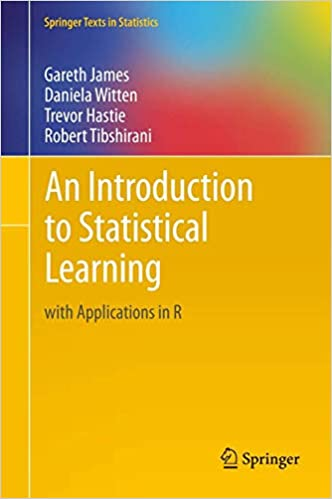
\includegraphics[scale=0.3]{Figuras/slide03_01.jpg}
\end{figure}
Capítulo 2:  Statistical Learning.
\vone
\scriptsize

An Introduction to Statistical Learning: with Applications in R. G. James, D. Witten, T. Hastie, and R. Tibshirani. Springer, 2013.

\end{ftst}

%=====

\begin{ftst}{Visão geral}{{Aprendizado Estatístico}}
\justifying
A aprendizagem estatística refere-se a um vasto conjunto de ferramentas para a compreensão de dados.
\vone
Essas ferramentas podem ser classificadas como supervisionadas ou não supervisionadas. 
\vone
\begin{itemize}
    \item Em termos gerais, o aprendizado estatístico supervisionado envolve a construção de um modelo estatístico para prever ou estimar uma saída com base em uma ou mais entradas. 
    \item Com o aprendizado estatístico não supervisionado, existem entradas, mas nenhuma saída de supervisão; no entanto, podemos aprender relacionamentos e estruturas a partir de tais dados.
\end{itemize}
\end{ftst}

%=====

\begin{ftst}{Visão geral}{{Aprendizado Estatístico}}
\justifying
Exemplo de problema onde o \textbf{aprendizado supervisionado} é usado:
\vone

\begin{figure}
    \centering
    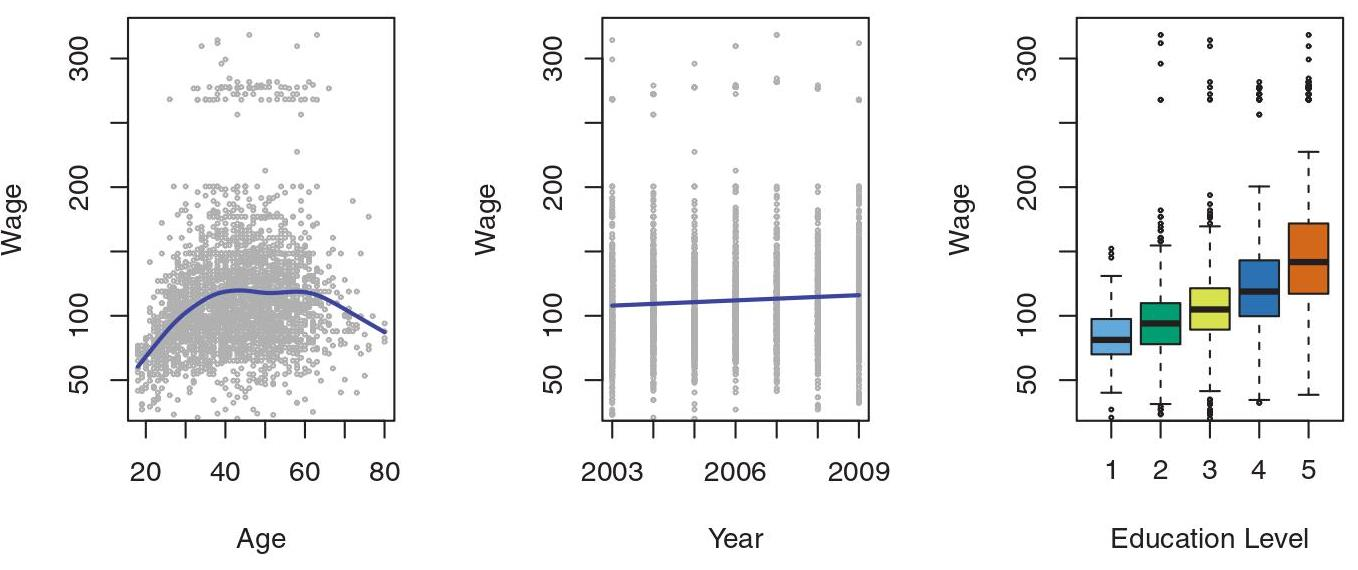
\includegraphics[scale=0.9]{Figuras/slide03_02.jpg}
\end{figure}
\end{ftst}

%=====

\begin{ftst}{Visão geral}{{Aprendizado Estatístico}}
\justifying
Exemplo de problema onde o \textbf{aprendizado não supervisionado} é usado:
 
\vone
\begin{figure}
    \centering
    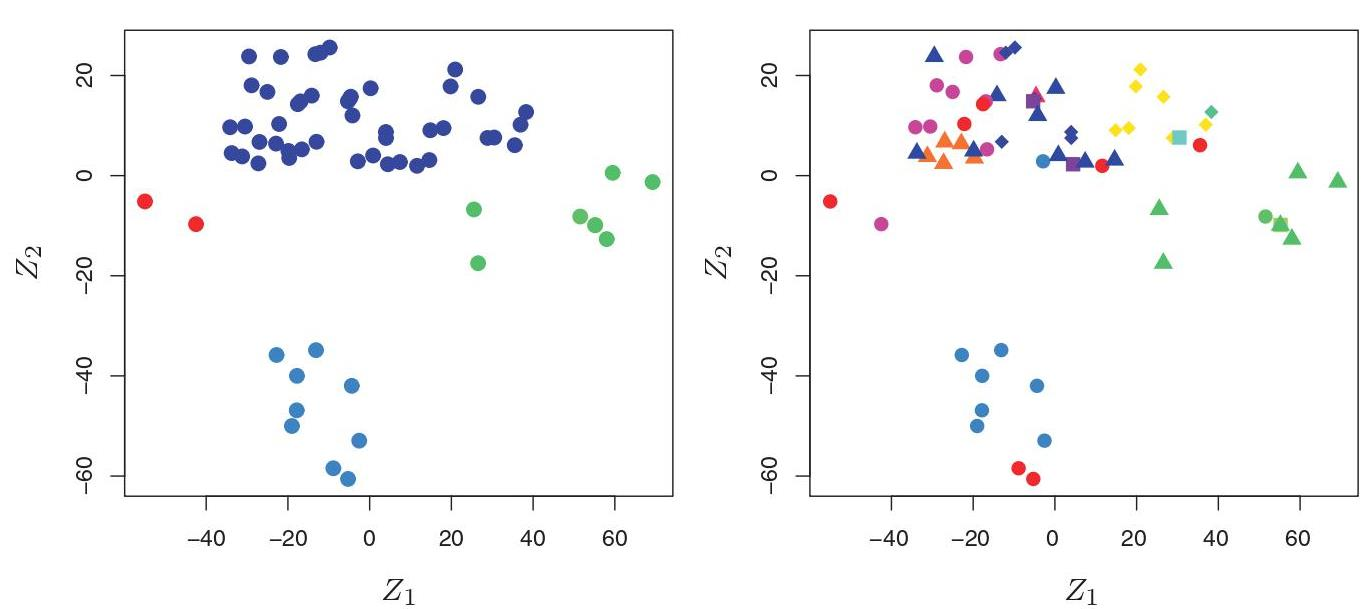
\includegraphics[scale=0.8]{Figuras/slide03_03.jpg}
\end{figure}

Isso é conhecido como um problema de cluster e, ao contrário do exemplo anterior, aqui não estamos tentando prever uma variável de saída.
\end{ftst}

%=====


\begin{ftst}{Visão geral}{{Aprendizado Estatístico}}
\justifying
Suponha que sejamos consultores estatísticos contratados por um cliente para aconselhar sobre como melhorar as vendas de um determinado produto.
\vone
O conjunto de dados de publicidade consiste nas vendas desse produto em 200 mercados diferentes, juntamente com orçamentos de publicidade para o produto em cada um desses mercados para três meios de comunicação diferentes: TV, rádio e jornal.
\vone
Se determinarmos que existe uma associação entre publicidade e vendas, podemos instruir nosso cliente a ajustar os orçamentos de publicidade, aumentando indiretamente as vendas.

\end{ftst}

%=====

\begin{ftst}{Visão geral}{{Aprendizado Estatístico}}
\justifying
Os orçamentos de publicidade são variáveis de entrada, enquanto a entrada de vendas é uma variável de saída.

\begin{figure}
    \centering
    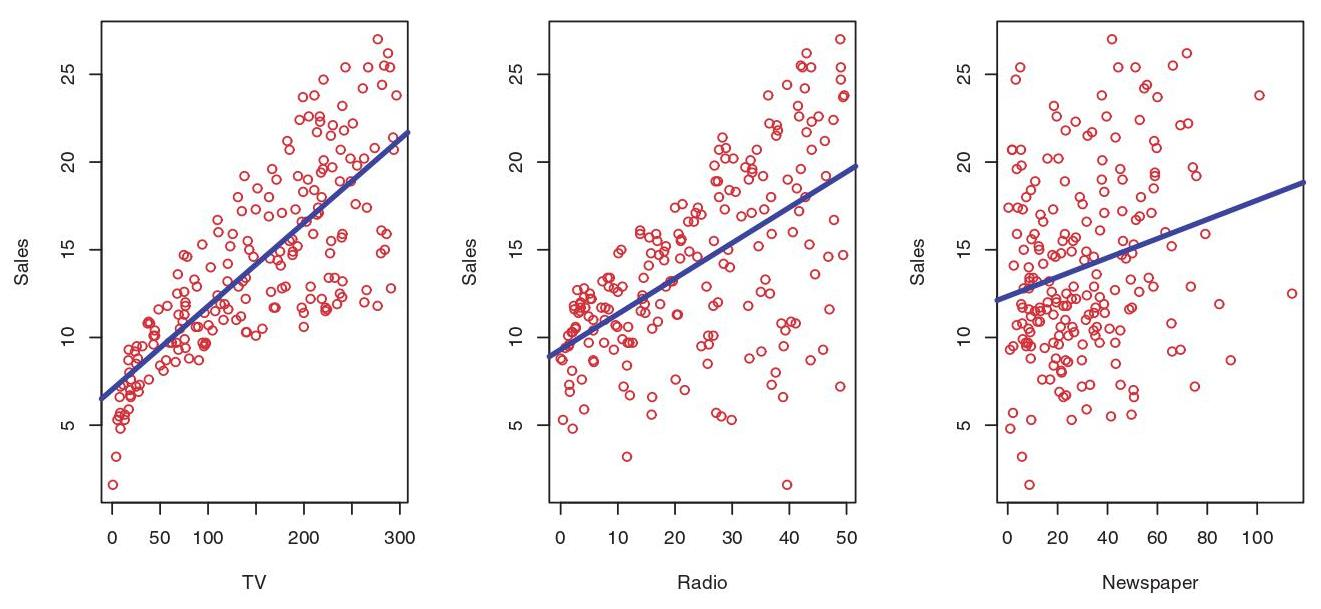
\includegraphics[scale=0.7]{Figuras/slide03_04.jpg}
\end{figure}
\small
Variáveis de entrada ou variáveis independentes: são os orçamentos de publicidade (com TV, Rádio e Jornal). Vamos chamá-las de $X_1$, $X_2$ e $X_3$.
\vone
Variável de saída ou variável dependente: são as vendas. Vamos chamá-la de $Y$.
\end{ftst}

%=====

\begin{ftst}{Visão geral}{{Aprendizado Estatístico}}
\justifying
\textbf{Objetivo:} desenvolver um modelo preciso que possa ser usado para prever vendas com base nos três orçamentos de mídia.
\vone
Para isso, podemos assumir que existe uma relação entre $Y$ e $X$:

\vone
\begin{equation}
    Y = f(X) + \epsilon
\end{equation}
\vone
Onde:
\vone
- $f(X)$ é uma função desconhecida de $X_1, X_2 e X_3$.

- $\epsilon$ é um erro aleatório, independente de $X$ e com média zero.
\end{ftst}

%=====

\begin{ftst}{Visão geral}{{Aprendizado Estatístico}}
\justifying

Exemplo: o gráfico sugere que alguém pode ser capaz de prever a renda usando anos de educação.

\begin{figure}
    \centering
    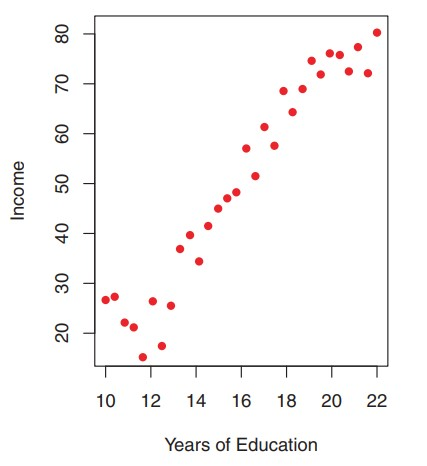
\includegraphics[scale=0.3]{Figuras/slide03_05.jpg}
\end{figure}

No entanto, a função $f$ que conecta a variável de entrada à variável de saída é geralmente desconhecida e devemos estimá-la com base nos pontos observados.


\end{ftst}

%=====

\begin{ftst}{Visão geral}{{Aprendizado Estatístico}}
\justifying
Aqui, a curva azul mostra a função $f$ e as linhas verticais representam os termos de erro ($\epsilon$).

\begin{figure}
    \centering
    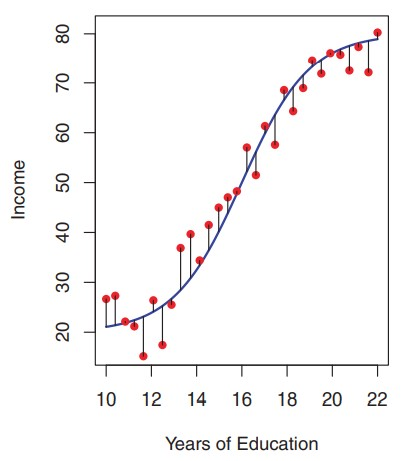
\includegraphics[scale=0.3]{Figuras/slide03_06.jpg}
\end{figure}

Notamos que algumas das 30 observações estão acima da curva azul e algumas abaixo dela, ou seja, o erro médio é aproximadamente 0.


\end{ftst}

%=====

\begin{ftst}{Visão geral}{{Aprendizado Estatístico}}
\justifying
Em geral, a função $f$ pode envolver mais de uma variável de entrada.
\vone
Nesse exemplo, representamos a renda em função dos anos de educação e da idade.
\vone
Agora, $f$ é uma superfície bidimensional que deve ser estimada com base nos dados observados.

\begin{figure}
    \centering
    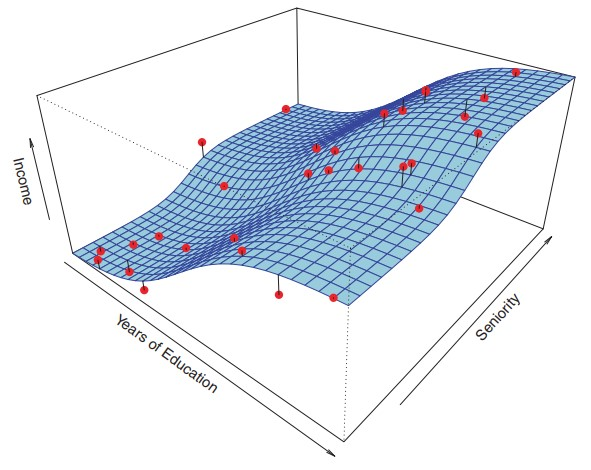
\includegraphics[scale=0.3]{Figuras/slide03_07.jpg}
\end{figure}



\end{ftst}

%=====

\begin{ftst}{Visão geral}{{Aprendizado Estatístico}}
\justifying
Em essência, a aprendizagem estatística se refere a um conjunto de abordagens para estimar $f$.
\vone
\textbf{Por que desejamos estimar $f$?}
\vone
\begin{itemize}
    \item Para fazer previsões para $Y$.
    \item Para fazer inferências, ou seja, para entender como $Y$ é afetado quando $X_1, ..., X_p$ mudam.
\end{itemize}
\end{ftst}

%=====

\begin{ftst}{Visão geral}{{Aprendizado Estatístico}}
\justifying
\textbf{Como podemos estimar $f$?}
\vone
\begin{itemize}
    \item Métodos paramétricos: envolvem uma abordagem baseada em modelo.
    \item Métodos não-paramétricos: não fazem suposições explícitas sobre a forma de $f$. 
\end{itemize}

\end{ftst}

%=====

\begin{ftst}{Métodos paramétricos}{{Aprendizado Estatístico}}
\justifying
Primeiro, fazemos uma suposição sobre a forma de $f$. Por exemplo, uma suposição muito simples é que $f$ é linear em $X$:
\begin{equation}
    f(X) = \beta_0 + \beta_1 X_1 + \beta_2 X_2 + \ldots + \beta_p X_p
\end{equation}
\vone
Uma vez que assumimos que $f$ é linear, o problema de estimar $f$ é bastante simplificado, pois precisamos estimar apenas os coeficientes $\beta_0, \beta_1, ..., \beta_p$.
\vone
Após a seleção de um modelo, precisamos de um procedimento que use os dados de treinamento para ajustar ou treinar o modelo.

\end{ftst}

%=====

\begin{ftst}{Métodos paramétricos X não-paramétricos}{{Aprendizado Estatístico}}
\justifying
\begin{itemize}
    \item Ao evitar a suposição de uma forma específica para  $f$, os métodos não-paramétricos têm o potencial de ajustar com precisão uma faixa mais ampla de formas possíveis para $f$.
    \item Qualquer abordagem paramétrica traz a possibilidade de que a forma usada para estimar $f$ seja muito diferente da $f$ verdadeira, caso em que o modelo resultante não se ajustará bem aos dados.
    \item Mas abordagens não paramétricas sofrem de uma grande desvantagem: como não reduzem o problema de estimar $f$ para um pequeno número de parâmetros, é necessário um número muito grande de observações (muito mais do que o normalmente necessário para uma abordagem paramétrica) para obter uma estimativa precisa de $f$.

\end{itemize}

\end{ftst}


%=====

\begin{ftst}{Métodos paramétricos X não-paramétricos}{{Aprendizado Estatístico}}
\vone
\vone
\begin{figure}[!htb]
    \centering
    \begin{minipage}{.5\textwidth}
        \centering
        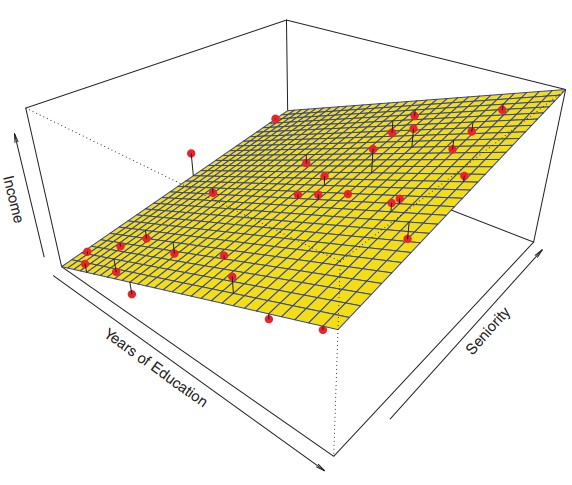
\includegraphics[scale=0.3]{Figuras/slide03_08.jpg}
        \caption{Paramétrico}
        \label{fig:01}
    \end{minipage}%
    \begin{minipage}{0.5\textwidth}
        \centering
        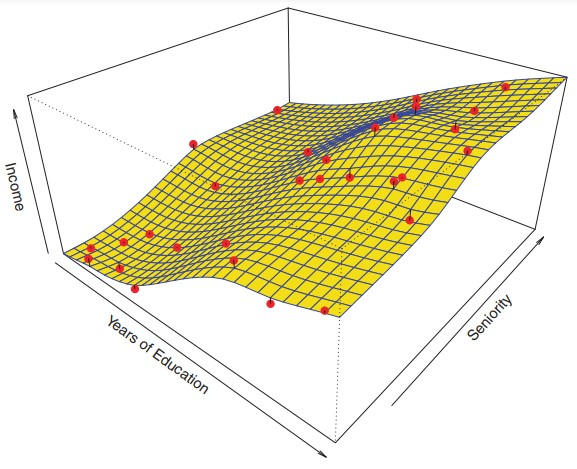
\includegraphics[scale=0.3]{Figuras/slide03_09.jpg}
        \caption{Não-paramétrico}
        \label{fig:02}
    \end{minipage}
\end{figure}

\end{ftst}


%=====

\begin{ftst}{O \textit{trade-off} entre precisão e interpretabilidade}{{Aprendizado Estatístico}}
\begin{figure}
    \centering
    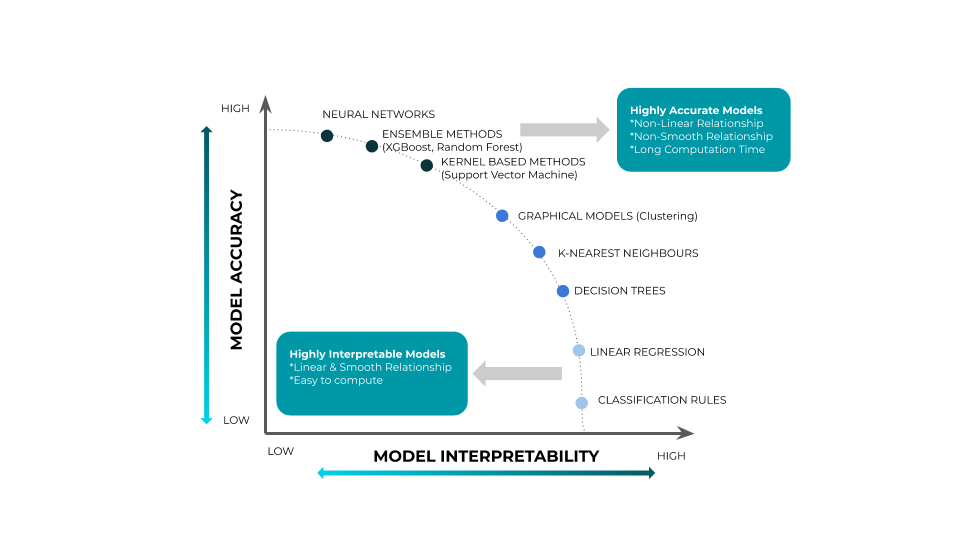
\includegraphics[trim=120 60 80 80,clip,scale=0.4]{Figuras/slide03_10.png}
\end{figure}
\small
Por que escolheríamos usar um método mais restritivo em vez de uma abordagem mais flexível?
\end{ftst}

%=====

\begin{ftst}{Aprendizado Supervisionado}{{Aprendizado Estatístico}}
\textbf{Regressão X Classificação}
\begin{figure}
    \centering
    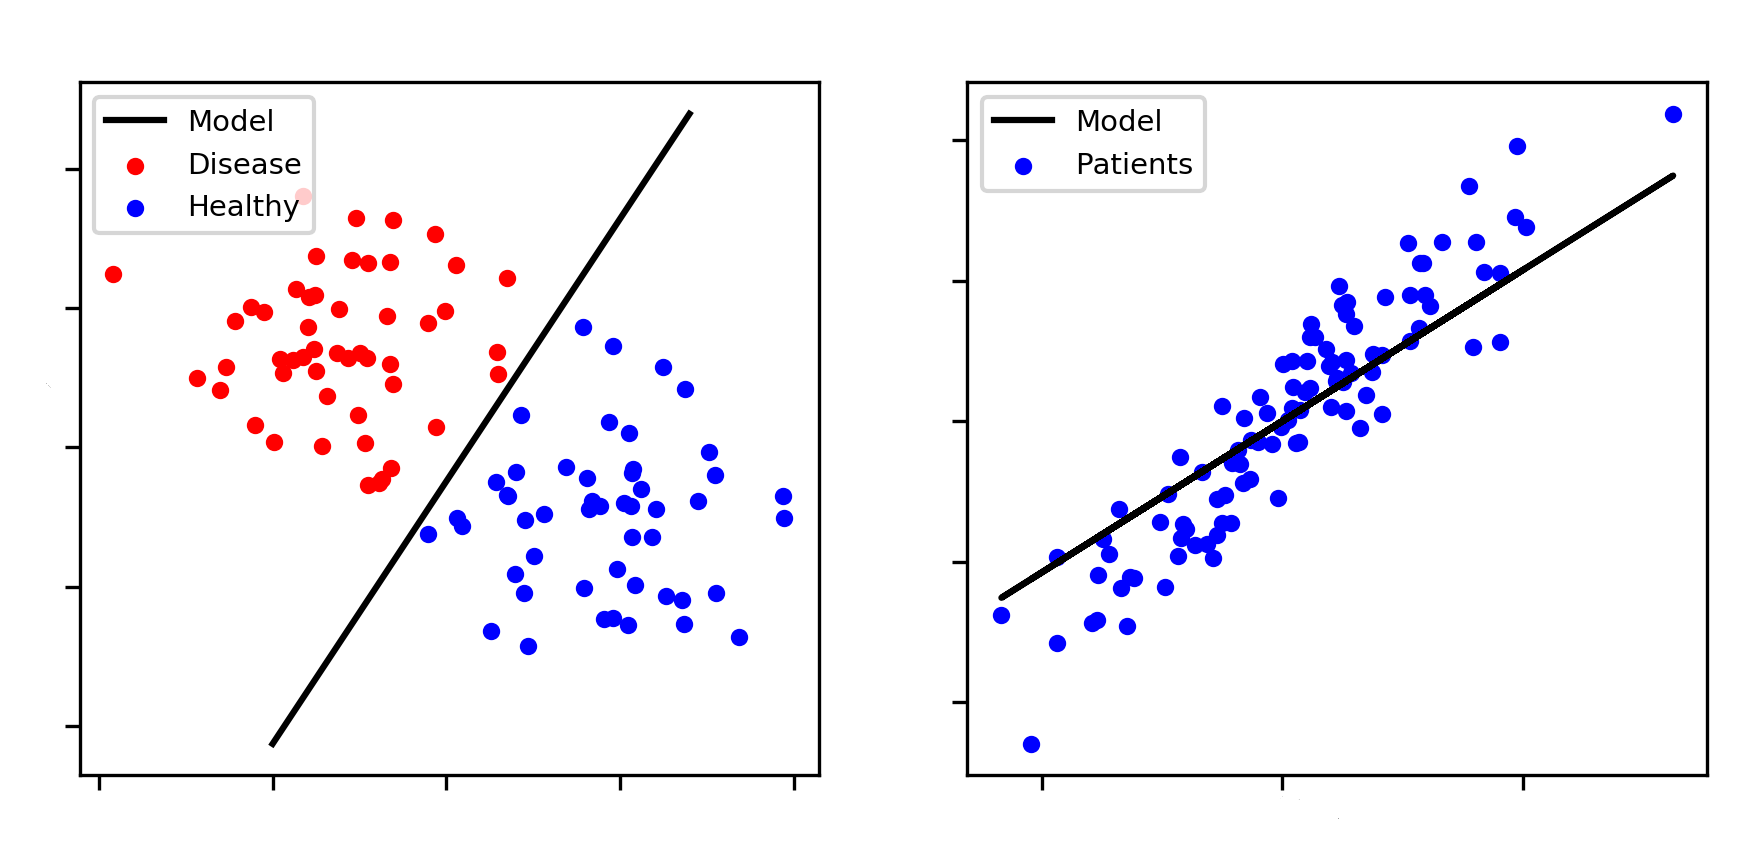
\includegraphics[scale=0.25]{Figuras/slide03_11.png}
\end{figure}
\end{ftst}

%=====

\begin{ftst}{Avaliação da precisão do modelo}{{Aprendizado Estatístico}}
\justifying
Por que é necessário introduzir tantas abordagens diferentes de aprendizagem estatística, em vez de apenas um único método melhor? 
\vone
Não há almoço grátis em estatística: nenhum método domina todos os outros sobre todos os conjuntos de dados possíveis.
\vone
Portanto, é uma tarefa importante decidir, para qualquer conjunto de dados, qual método produz os melhores resultados. 
\vone
Selecionar a melhor abordagem pode ser uma das partes mais desafiadoras do desempenho do aprendizado estatístico na prática.
\end{ftst}

%=====

\begin{ftst}{Medindo a qualidade do ajuste}{{Aprendizado Estatístico}}
\justifying
A fim de avaliar o desempenho de um método de aprendizado estatístico em um determinado conjunto de dados, precisamos de alguma forma para medir o quão bem suas previsões realmente correspondem aos dados observados.
\vone
Ou seja, precisamos quantificar até que ponto o valor de resposta previsto para uma determinada observação está próximo do valor de resposta verdadeiro para essa observação.
\vone
Para minimizar o erro de teste esperado, precisamos selecionar um método de aprendizado estatístico que alcance simultaneamente baixa variância e baixo viés.
\end{ftst}

%=====

\begin{ftst}{O \textit{trade-off} entre viés e variância}{{Aprendizado Estatístico}}
\justifying
\textbf{Variância:}
\begin{itemize}
    \item A variância refere-se à mudança que $\hat{f}$ sofreria se a estimássemos usando um conjunto de dados de treinamento diferente. 
    \item Como os dados de treinamento são usados para se ajustar ao método estatístico de aprendizado, diferentes conjuntos de dados de treinamento resultam em um $\hat{f}$ diferente. 
    \item Idealmente, a estimativa para $f$ não deve variar muito entre os conjuntos de treinamento. 
    \item Quando um método tem alta variância, pequenas alterações nos dados de treinamento podem resultar em grandes alterações em $\hat{f}$.

\end{itemize}
\end{ftst}

%=====

\begin{ftst}{O \textit{trade-off} entre viés e variância}{{Aprendizado Estatístico}}
\justifying
\textbf{Viés:}
\begin{itemize}
    \item O viés refere-se ao erro.
    \item Por exemplo: a regressão linear assume que há uma relação linear entre $Y$ e $X_1, X_2, \cdot, X_p$. É improvável que qualquer problema da vida real realmente tenha uma relação linear tão simples e, portanto, a realização da regressão linear resultará, sem dúvida, em algum viés na estimativa de $f$.
\end{itemize}
\end{ftst}

%=====

\begin{ftst}{O \textit{trade-off} entre viés e variância}{{Aprendizado Estatístico}}
\justifying
\begin{figure}
    \centering
    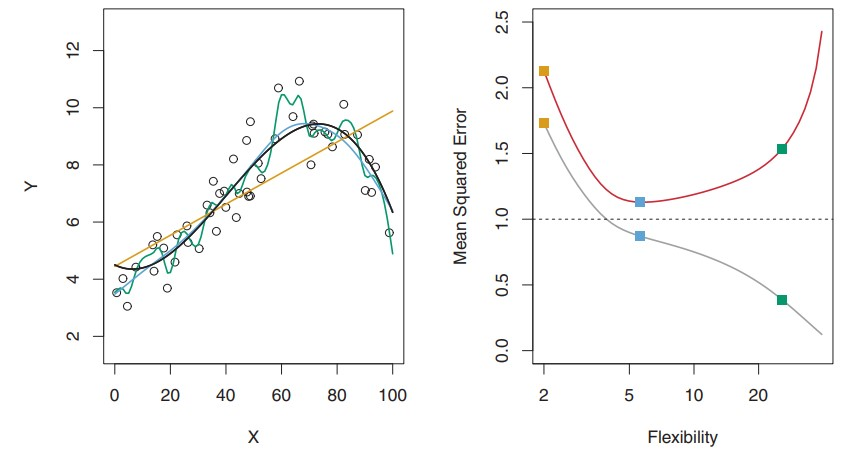
\includegraphics[scale=0.35]{Figuras/slide03_12.jpg}
\end{figure}
\small
Gráfico à direita:

- Curva vermelha: erro de teste.

- Curva cinza: erro de treino.

\end{ftst}

%=====

\begin{ftst}{O \textit{trade-off} entre viés e variância}{{Aprendizado Estatístico}}
\justifying
\textit{\textbf{Underfitting: }}ocorre em modelos com alto viés e baixa variância.

Exemplo: linha amarela.
\vone
\textit{\textbf{Overfitting:}} ocorre em modelos com baixo viés e alta variância.

Exemplo: curva verde.

\begin{figure}
    \centering
    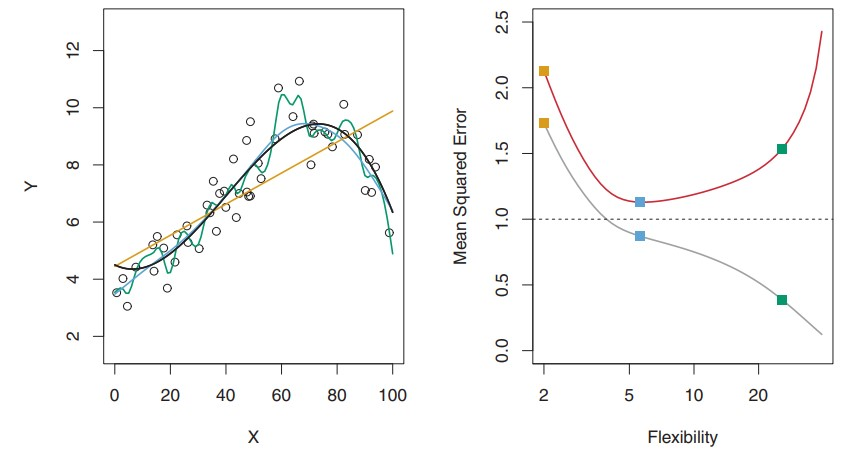
\includegraphics[scale=0.4]{Figuras/slide03_12.jpg}
\end{figure}

\end{ftst}

%=====

\begin{ftst}{O \textit{trade-off} entre viés e variância}{{Aprendizado Estatístico}}


\begin{figure}
    \centering
    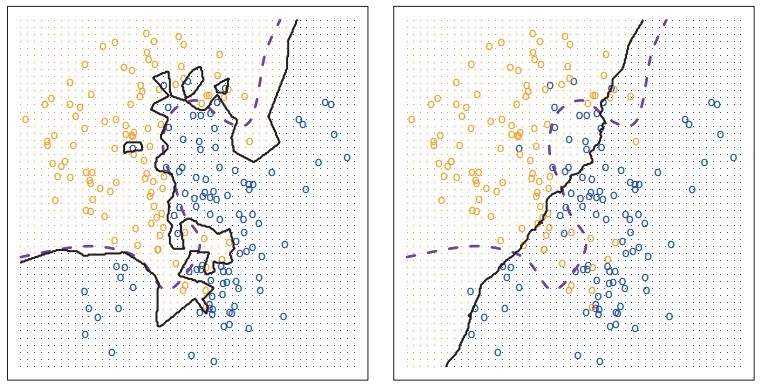
\includegraphics[scale=0.4]{Figuras/slide03_13.jpg}
\end{figure}

\end{ftst}

%=====

\end{document}